
\documentclass[
	10.0pt, % Tamanho padrão da fonte
	% t, % Alinhar verticalmente ao topo
	% aspectratio=169, % Definir proporção 16:9
]{beamer}

% Caminho para imagens
\graphicspath{{img/}}

% Pacotes adicionais
\usepackage[alf]{abntex2cite} % Citações ABNT
\usepackage{booktabs} % Linhas de tabela aprimoradas
\usepackage{raleway} % Fonte
%----------------------------------------------------------------------------------------
%	SELEÇÃO DE LAYOUT E CORES
%----------------------------------------------------------------------------------------

\usetheme{Boadilla} % Tema de layout

% Definição de cores personalizadas
\definecolor{primaryColor}{RGB}{20,45,105} % Cor primária
\definecolor{secondaryColor}{RGB}{0,100,160} % Cor secundária

% Aplicação das cores no tema
\setbeamercolor{structure}{fg=primaryColor}
\setbeamercolor{palette primary}{bg=primaryColor, fg=white}
\setbeamercolor{palette secondary}{bg=secondaryColor, fg=white}
\setbeamercolor{title}{bg=primaryColor, fg=white} % Cor do título principal

% Cores no cabeçalho
\setbeamercolor{headline}{bg=secondaryColor, fg=white}
\setbeamercolor{section in head/foot}{bg=primaryColor, fg=white}
\setbeamercolor{subsection in head/foot}{bg=secondaryColor, fg=white}

% Configurações de cores para o rodapé
\setbeamercolor{author in head/foot}{bg=primaryColor, fg=white} % Nome
\setbeamercolor{title in head/foot}{bg=secondaryColor, fg=white} % Título
\setbeamercolor{date in head/foot}{bg=primaryColor, fg=white} % Ano
\setbeamercolor{page number in head/foot}{bg=primaryColor, fg=white} % Página

% Temas internos e externos
\useinnertheme{circles} % Tema interno
\useoutertheme{miniframes} % Tema externo
\setbeamertemplate{navigation symbols}{} % Remove símbolos de navegação

%----------------------------------------------------------------------------------------
%	INFORMAÇÕES DA APRESENTAÇÃO
%----------------------------------------------------------------------------------------

\title[Introdução ao Machine Learning]{Introdução ao Machine Learning\\ Aplicado com Scikit-learn e NumPy}
\author[GET-ENGCOMP]{Igor Correa Trifilio Campos, dá certo mesmo?, Filipe Moreira Vidal, Vitor Hugo Coradini} 
\institute[]{GET Engenharia Computacional} 
\date[2024]{} 

%----------------------------------------------------------------------------------------

\begin{document}

%----------------------------------------------------------------------------------------
%	SLIDE DE TÍTULO
%----------------------------------------------------------------------------------------

\begin{frame}
    \begin{figure}
        
\includegraphics[width=0.30\linewidth]{img/GETlogo_azul.png}
    \end{figure}
    \titlepage % Exibe o slide de título
\end{frame}

%----------------------------------------------------------------------------------------
%	SLIDE DE ÍNDICE
%----------------------------------------------------------------------------------------

\begin{frame}
    \frametitle{Estrutura do Minicurso} % Título do slide
    \tableofcontents % Exibe o índice
\end{frame}

%----------------------------------------------------------------------------------------
%	SEÇÕES DO CORPO DA APRESENTAÇÃO
%----------------------------------------------------------------------------------------

\section{Introdução} % Seções são adicionadas para organizar sua apresentação em blocos discretos, todas as seções e subseções são automaticamente exibidas no índice como uma visão geral da apresentação, mas NÃO são exibidas como slides separados.

%------------------------------------------------

\begin{frame}
    \frametitle{Introdução à Machine Learning}
    
    Processo de ensinar um computador a fazer previsões ou tomar decisões a partir de dados, identificando padrões ou regularidades.

    \vspace{0.5cm}

    \textbf{Exemplos:}
    \begin{enumerate}
        \setlength{\itemsep}{10pt}
        \item Recomendação de Produtos (ex.: Netflix, Amazon)
        \item Reconhecimento de Imagens (ex.: diagnóstico médico, reconhecimento facial)
        \item Previsão de Séries Temporais (ex.: previsão de demanda, previsão de vendas)
    \end{enumerate}
\end{frame}

\begin{frame}
	\frametitle{Introdução à Machine Learning}
    \vspace{0.2cm}
     \textbf{Fluxo de Trabalho}
     \vspace{0.2cm}
    \begin{itemize}
        \item Pré Processamento
        \item Treinamento
        \item Validação
    \end{itemize}
     
    \begin{center}
        \centering
        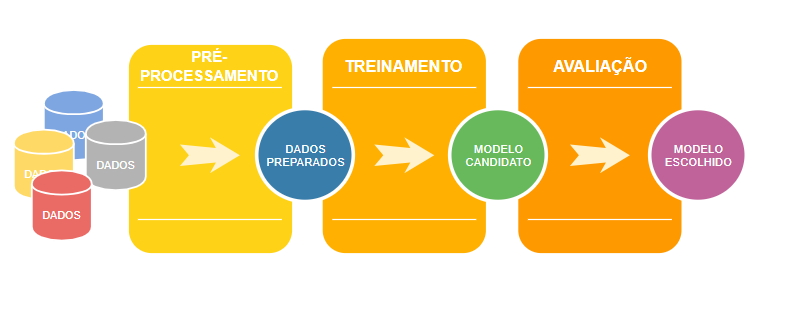
\includegraphics[width=1.0\linewidth]{img/introaml.png}
    \end{center}
\end{frame}

\begin{frame}
    \frametitle{Desenvolvimento no Colab}
    \centering
    
    Link para o acesso ao minicurso no colab\\ está no site do GET-EngComp:

    \vspace{0.5cm}
    
    \href{https://www2.ufjf.br/getengcomp/}{www2.ufjf.br/getengcomp/}        
\end{frame}
\section{Pré-processamento} 

\begin{frame}
    \frametitle{Pré-processamento de Dados}
    \begin{itemize} 
        \item Dados reais podem conter valores ausentes, variáveis desbalanceadas ou ruídos.
        \item Preparação, organização e estruturação dos dados.
        \item Modelos de ML requerem dados bem formatados.
    \end{itemize}

    \begin{center}
    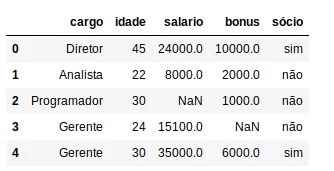
\includegraphics[width=0.6\linewidth]{img/tabelaintropre.jpg}
    \end{center}

\end{frame}

\begin{frame}
    \frametitle{Técnicas}
    \begin{itemize} 
        \item Codificação de variáveis categóricas 
        \item Padronização
        \item Normalização
        \item Divisão dos dados
    \end{itemize}
\end{frame}

\begin{frame}
    \frametitle{Codificação de variáveis categóricas}
    Utilizadas para converter variáveis categóricas em uma forma numérica que possa ser utilizada por modelos de Machine Learning.

    \vspace{0.3cm}
    
    \begin{itemize}
        \item Label Encoder.
        \item One Hot Encoder.
    \end{itemize}
\end{frame}

\begin{frame}{Label Encoder}
    \begin{itemize}
        \item Converte variáveis categóricas em valores inteiros.
        \item Ideal para categorias com uma ordem (variáveis ordinais).
    \end{itemize}

    \begin{center}
    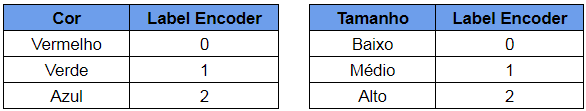
\includegraphics[width=0.8\linewidth]{img/LabelEncoder2.png}
    \end{center}

    \begin{center}
    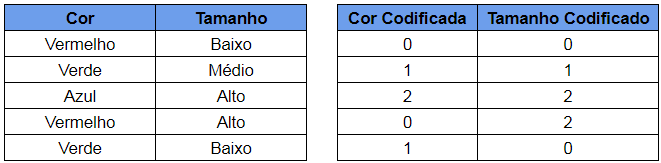
\includegraphics[width=0.8\linewidth]{img/LabelEncoder.png}
    \end{center}
\end{frame}

\begin{frame}{One Hot Encoder}
    
    \begin{itemize}
        \item Cria uma nova variável binária (0 ou 1) para cada categoria única da variável original.
        \item Ideal para um número reduzido de categorias e variáveis nominais.
    \end{itemize}
    
    \begin{center}
    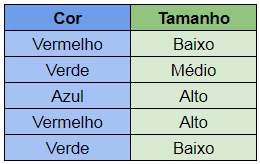
\includegraphics[width=0.3\linewidth]{img/One Hot 2.png}
    \end{center}

    \begin{center}
    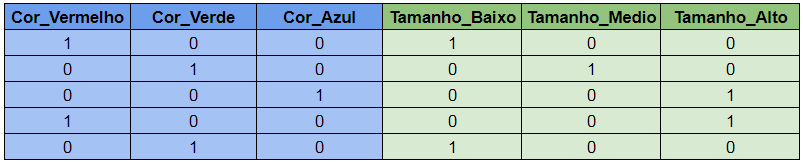
\includegraphics[width=0.8\linewidth]{img/One Hot.png}
    \end{center}
\end{frame}


\begin{frame}
    \frametitle{Padronização (Z-Score)}
    \begin{itemize}
    \setlength{\itemsep}{6pt}
        \item  Os dados são transformados de acordo com a distribuição estatística.
        \item Utiliza a Média e o Desvio Padrão.
        \item Menos sensível a outliers (valores extremos).
        \item Pode resultar em valores negativos.
    \end{itemize}
    
    \begin{center}
        \[
        X' = \frac{x - \mu}{\sigma}
        \]
    \end{center}
    
\end{frame}

\begin{frame}{Padronização}
    Padronização para o exemplo anterior
    \begin{itemize}
        \item Média (\(\mu\)): 41.0
        \item Desvio padrão (\(\sigma\)): 19.97
    \end{itemize}
    \vspace{0.3cm}
    \centering
  \begin{center}
    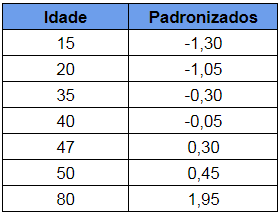
\includegraphics[width=0.4\linewidth]{img/Padronização.png}
    \end{center}
\end{frame}

\begin{frame}
    \frametitle{Normalização}
    
    \begin{itemize}
    \setlength{\itemsep}{10pt}
         \item Usado para reescalar os valores dos dados para que fiquem dentro de um intervalo específico, geralmente entre 0 e 1.
         \item Garante que todas as variáveis tenham a mesma escala.
         \item Evita que variáveis com valores maiores influenciem de forma desproporcional o modelo de Machine Learning.
     \end{itemize}
\end{frame}

\begin{frame}
    \frametitle{Normalização Min-Max}
    \begin{itemize}
    \setlength{\itemsep}{10pt}
         \item Um exemplo de normalização min-max é a conversão de idades de um grupo de pessoas para um intervalo entre 0 e 1.
        \item Se as idades são 15, 20, 35, 40 e 50 anos, o valor mínimo é 15 e o máximo é 50.
     \end{itemize}

    \begin{figure}[h!]
    \centering
    \begin{minipage}{0.45\textwidth}
        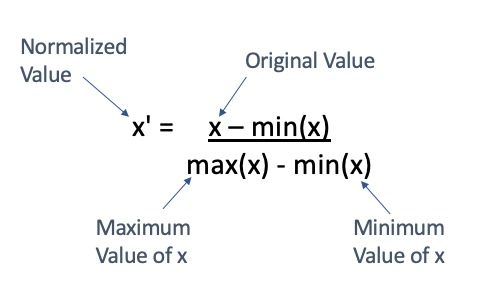
\includegraphics[width=1\linewidth]{img/minmax.jpg}
    \end{minipage}
    \begin{minipage}{0.45\textwidth}
        \centering
          \begin{center}
    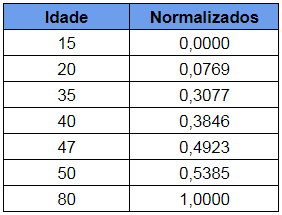
\includegraphics[width=0.8\linewidth]{img/Normalização.png}
    \end{center}
    \end{minipage}
    \end{figure}
     
\end{frame}

\begin{frame}
    \frametitle{Divisão dos dados}
    \begin{itemize}
    \setlength{\itemsep}{6pt}
        \item \textbf{Treinamento:} Usado para ajustar os parâmetros do modelo.
        \item \textbf{Validação:} Usado para avaliar o desempenho do modelo e dos hiperparâmetros durante o treinamento.
        \item \textbf{Teste:} Usado para avaliar a performance final do modelo em dados não vistos durante o treinamento.
    \end{itemize}

    \begin{figure}
        \centering
        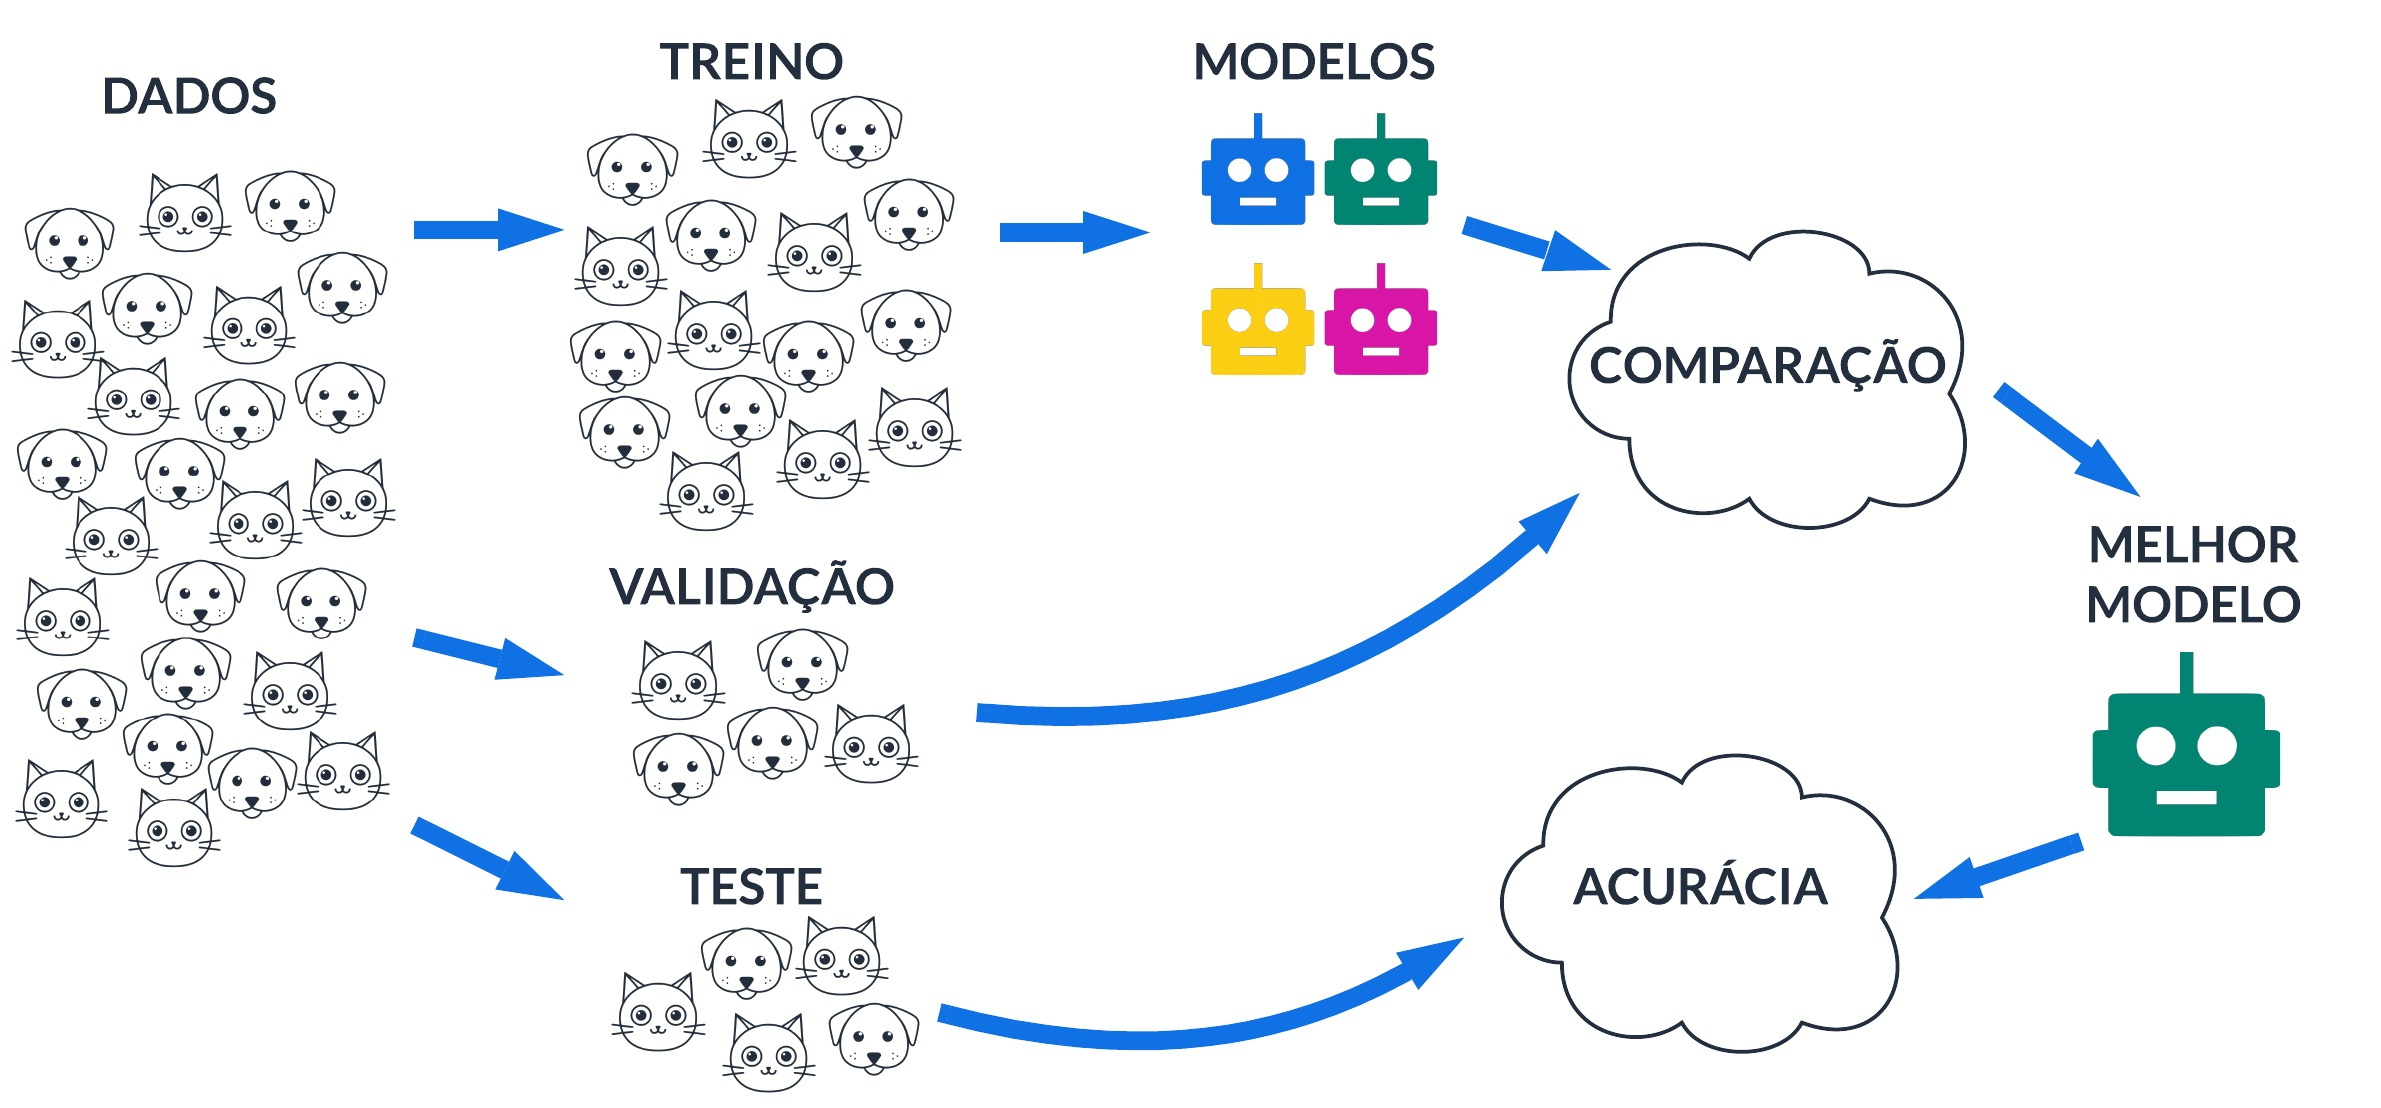
\includegraphics[width=0.7\linewidth]{img/image-ttv.png}
    \end{figure}
\end{frame}

\begin{frame}
    \frametitle{Divisão dos dados}

    Divisão mais comum dos dados que pode variar com base no desempenho do modelo:
    
    \vspace{0.3cm}
    
    \begin{itemize}
    \setlength{\itemsep}{6pt}
        \item \textbf{Treinamento:} 70\% - 80\% dos dados.
        \item \textbf{Validação:} 10\% - 15\% dos dados.
        \item \textbf{Teste:} 10\% - 15\% dos dados.
    \end{itemize}
\end{frame}
\section{Supervisionado} 

\begin{frame}
    \frametitle{Tipos de Aprendizado}
    \vspace{0.2cm}
     \textbf{Aprendizado Supervisionado x Não Supervisionado}
     \vspace{0.2cm}
     
     \begin{itemize}
         \item Supervisionado:
     \end{itemize}
         O modelo é treinado com dados rotulados, ou seja, dados em que já se sabe a resposta correta. (Regressão, Classificação).

    \vspace{0.3cm}
    
    \begin{itemize}
        \item Não Supervisionado:
     \end{itemize}
         O modelo encontra padrões ou grupos sem rótulos, ou seja, dados em que não se sabe a resposta correta. (Clustering/Agrupamento).
\end{frame}

\begin{frame}{Tipos de Aprendizado}
    \begin{center}
    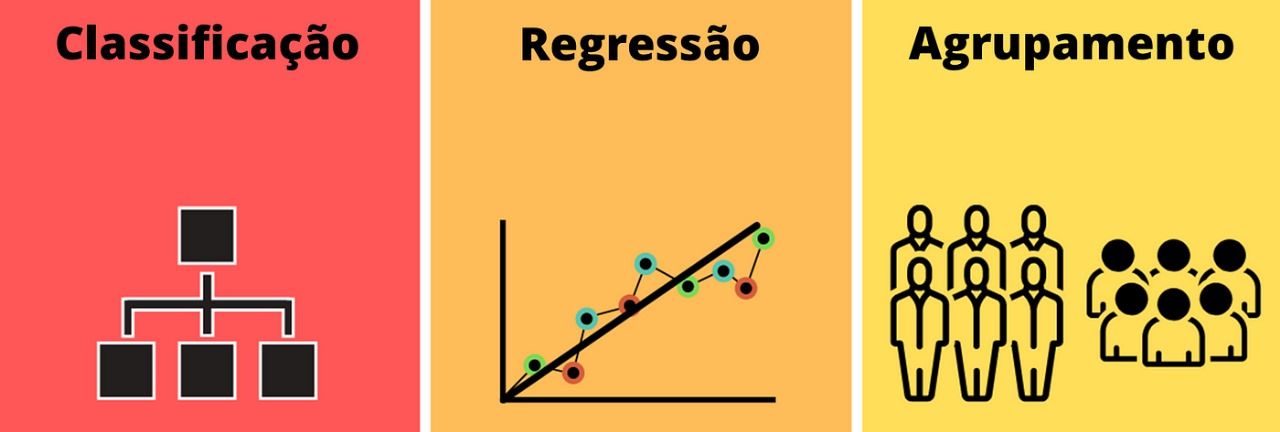
\includegraphics[width=1.0\linewidth]{img/TiposAprendizado.jpg}
    
    \end{center}
\end{frame}

\begin{frame}
    \frametitle{Aprendizado Supervisionado}
    \begin{figure}
        \centering
        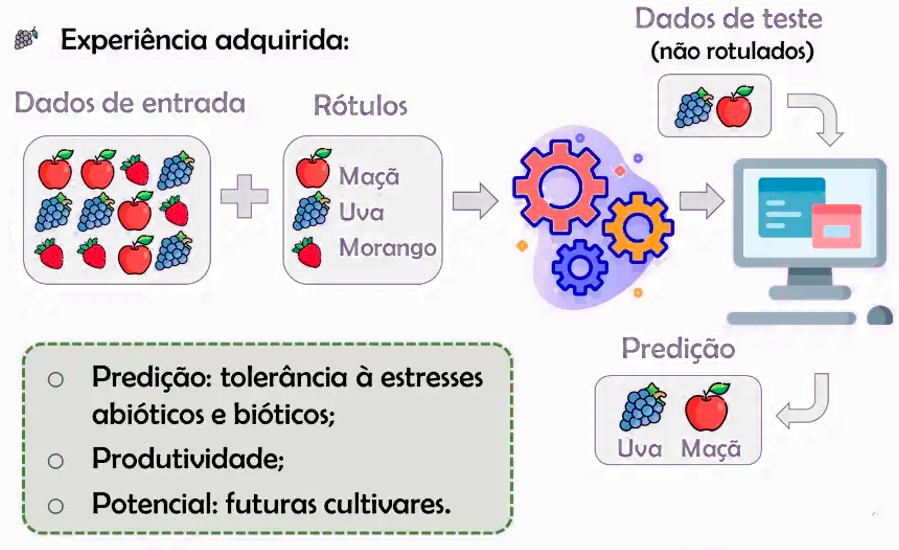
\includegraphics[width=1\linewidth]{img/supervisionado.png}
    \end{figure}
\end{frame}

\begin{frame}
    \frametitle{Classificação}
    \begin{itemize}
        \item Entender, reconhecer padrões e agrupar o conjunto de dados em categorias.
        \item Prever a categoria
    \end{itemize}
    \begin{figure}
        \centering
        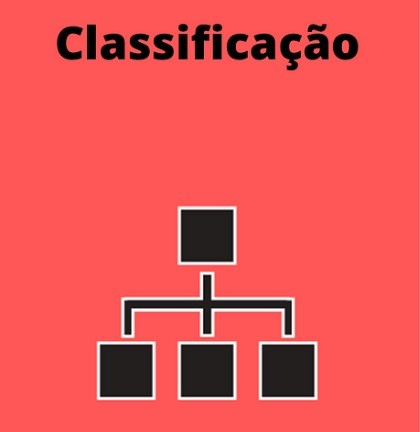
\includegraphics[width=0.3\linewidth]{img/Classificacao.jpg}
        \hspace{1cm}
        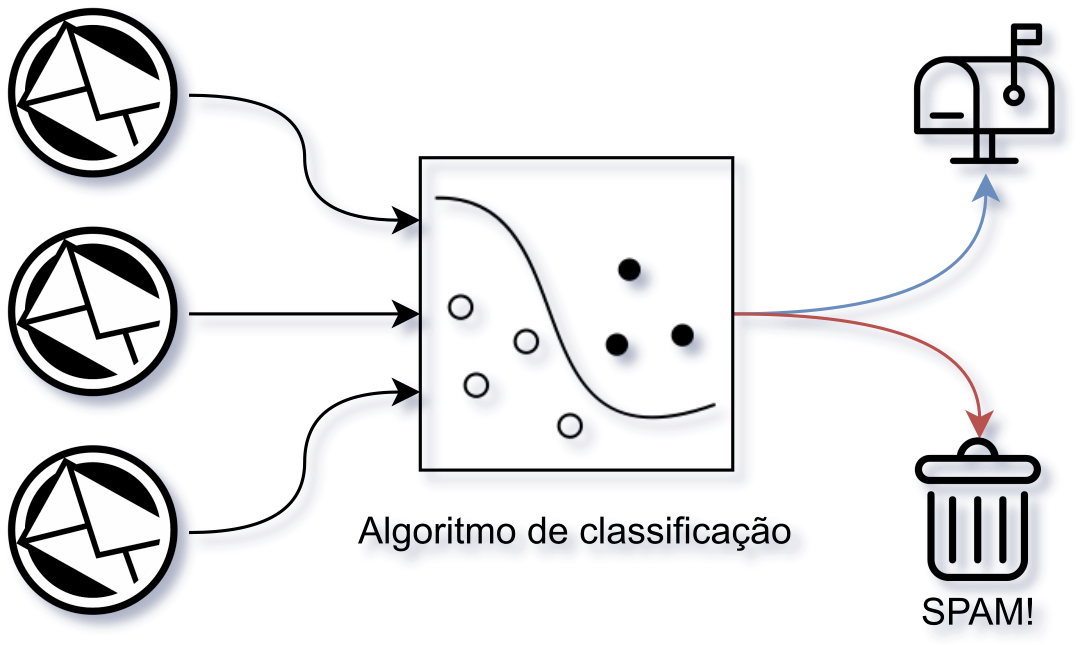
\includegraphics[width=0.5\linewidth]{img/ClassificacaoImagem.png}
    \end{figure}
\end{frame}

    \begin{frame}{Classificação}
    \textbf{Exemplos:}
    \begin{itemize}
        \item \textbf{Classificação de Gêneros Musicais:} Um modelo pode classificar uma música em múltiplos gêneros (ex.: rock e jazz).
        \item \textbf{Classificação de Rótulos de Produtos: }
        Atribuir um rótulo (como eletrônicos, vestuário, alimentos) a um produto com base em sua descrição.
        \item \textbf{Diagnóstico Médico: } Um classificador que utilize dados não observados de um paciente e classifique-o como doente ou não-doente.
    \end{itemize}
\end{frame}


\begin{frame}
    \frametitle{Matriz de Confusão}
    \begin{figure}
        \centering
        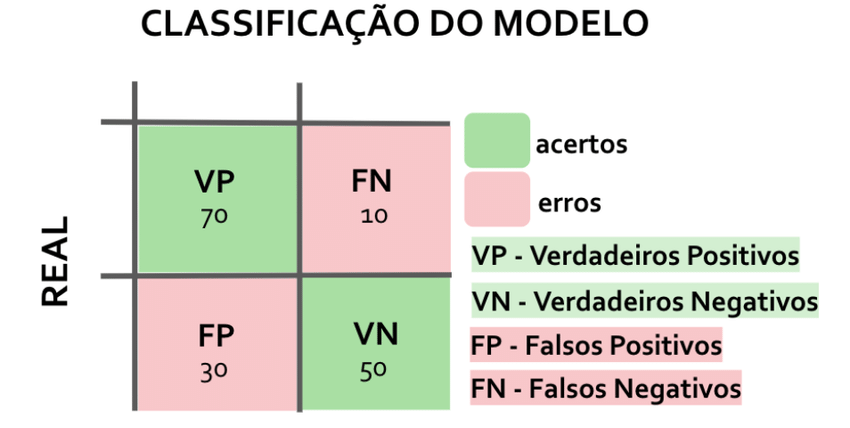
\includegraphics[width=0.8\linewidth]{img/MatrizConfusao.png}
    \end{figure}
    Usada para avaliar o desempenho de modelos de classificação.
\end{frame}

\begin{frame}
    \frametitle{Acurácia e Precisão}
    \textbf{Acurácia}
    \begin{itemize}
        \item Mede a proporção de \textbf{previsões corretas} (positivas e negativas) em relação ao total de previsões feitas.
    \end{itemize}

    \begin{center}
    \[
    Acuracia = \frac{VP + VN}{VP + VN + FP+ FN}
    \]
    \end{center}

    \textbf{Precisão}
    \begin{itemize}
        \item Mede a proporção de \textbf{previsões positivas} que estão realmente corretas.
        \item "Das vezes que o modelo previu positivo, quantas vezes ele estava certo?"
    \end{itemize}

    \begin{center}
    \[
    Precisao = \frac{VP}{VP + FP}
    \]
    \end{center}
    
\end{frame}

\begin{frame}
    \frametitle{Recall e F1 Score}
    \textbf{Recall}
    \begin{itemize}
        \item "Dos exemplos realmente positivos, quantos o modelo conseguiu prever corretamente?"
    \end{itemize}

    \begin{center}
    \[
    Recall = \frac{VP}{VP + FN}
    \]
    \end{center}

    \textbf{F1 Score}
    \begin{itemize}
        \item Média harmônica entre Precisão e Recall.
        \item Equilibra as duas métricas.
    \end{itemize}

    \begin{center}
    \[
    F1 Score = 2*\frac{Precisao*Recall}{Precisao + Recall}
    \]
    \end{center}
    
\end{frame}

\begin{frame}{Não devemos olhar só a acurácia!}
    \begin{figure}
        \centering
        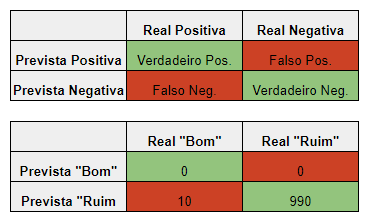
\includegraphics[width=0.5\linewidth]{img/MatrizComValores.png}
    \end{figure}
    \textbf{Dataset desbalanceado}
    \begin{itemize}
        \item 990 "Ruim"
        \item 10 "Bom"
    \end{itemize}

    \textbf{Modelo classifica tudo como "Ruim"}
    \begin{itemize}
        \item Acurácia: 99\%
        \item Recall: 0\%
    \end{itemize}
    
\end{frame}

\begin{frame}
    \frametitle{Regressão}
    \begin{itemize}
        \item Encontrar uma \textbf{função} que relacione as variáveis de entrada com a variável de saída.
    \end{itemize}
    \begin{figure}
        \centering
        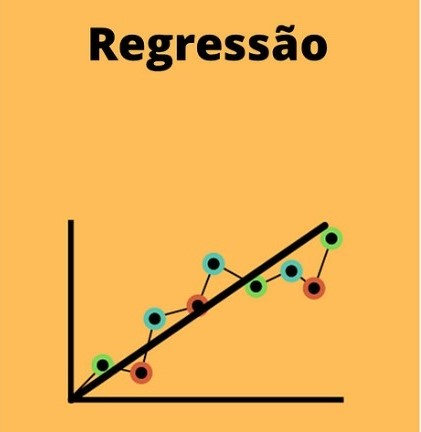
\includegraphics[width=0.3\linewidth]{img/Regressao.jpg}
        \hspace{0.2cm}
        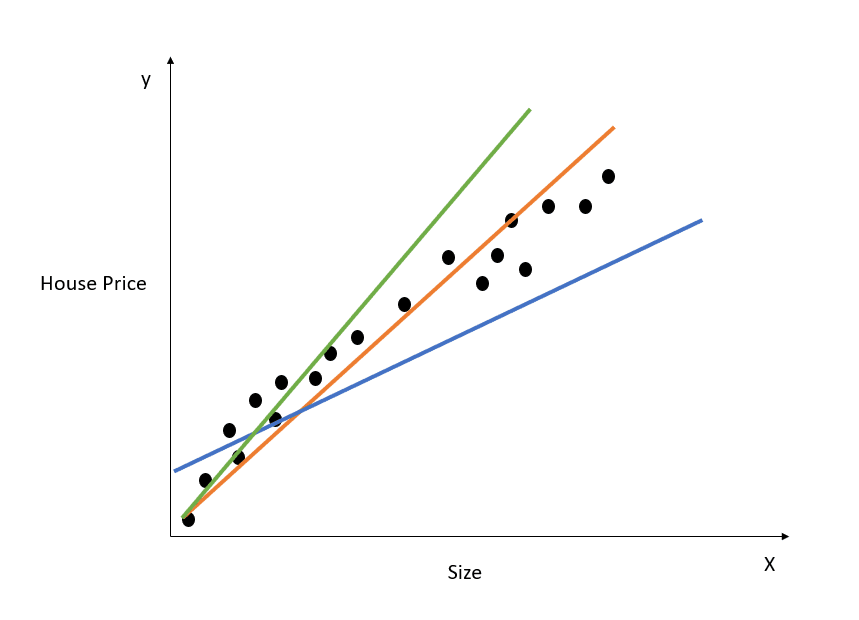
\includegraphics[width=0.5\linewidth]{img/RegressaoImagem.png}
    \end{figure}
    \begin{itemize}
        \item A linha \textbf{laranja} é a mais próxima de todos os pontos de dados mostrados.
        \item "Linha de Melhor Ajuste".
    \end{itemize}
\end{frame}

\begin{frame}
    \frametitle{Mean Absolut Error - MAE}
    \begin{itemize}
        \item Média da diferença entre o real e o previsto.
        \item valores maiores ou iguais a zero (módulo).
    \end{itemize}
    
   \begin{figure}
        \centering
        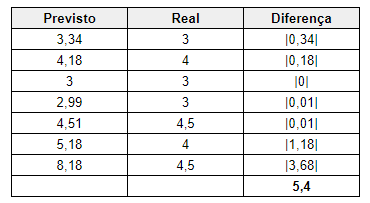
\includegraphics[width=0.6\linewidth]{img/TabelaMAE.png}
        \hspace{0.2cm}
        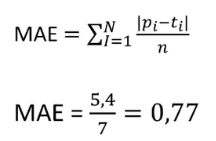
\includegraphics[width=0.3\linewidth]{img/MAEGabarito.png}
    \end{figure}
\end{frame}

\begin{frame}{Root Mean Squared Error - RMSE}
    \begin{itemize}
        \item Penaliza erros maiores de forma mais severa (quadrado).
        \item \textbf{Baixo RMSE:} O modelo está prevendo os valores reais com maior precisão.
        \item \textbf{Alto RMSE:} O modelo está cometendo erros significativos nas previsões.
    \end{itemize}
\end{frame}

\begin{frame}{Root Mean Squared Error - RMSE}

    \begin{figure}
        \centering
        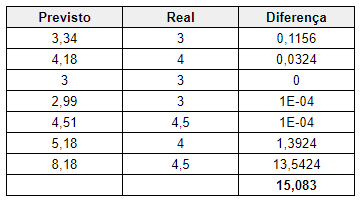
\includegraphics[width=0.6\linewidth]{img/TabelaRMSE.png}
        \hspace{0.2cm}
        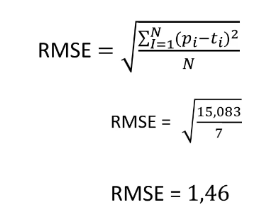
\includegraphics[width=0.4\linewidth]{img/RMSEGabarito.png}
    \end{figure}

\end{frame}

\begin{frame}{KNN}
    \begin{itemize}
        \item K-nearest neighbors, ou “K-vizinhos mais próximos”

        \item  Se os vizinhos mais próximos forem majoritariamente de uma classe, a amostra em questão será classificada nesta categoria.
        
    \end{itemize}
    \begin{figure}
        \centering
        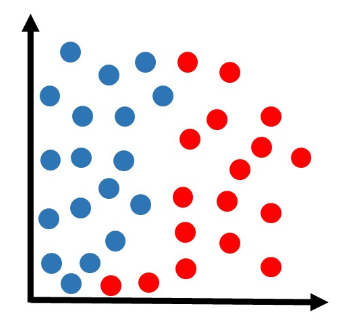
\includegraphics[width=0.20\linewidth]{img/KNN1.png}
    \end{figure}    
    
    \begin{figure}   
        \centering
        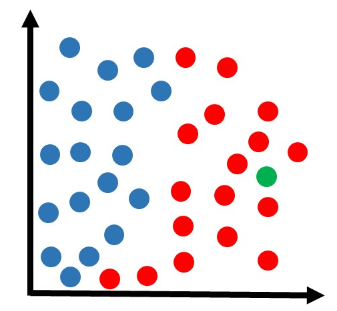
\includegraphics[width=0.20\linewidth]{img/KNN2.png}
        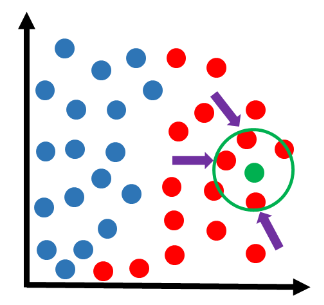
\includegraphics[width=0.20\linewidth]{img/KNN3.png}
        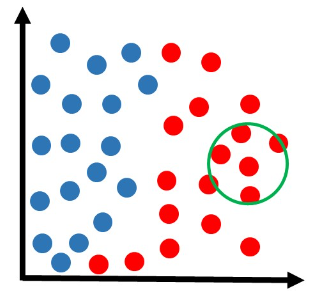
\includegraphics[width=0.20\linewidth]{img/KNN4.png}
    \end{figure}
\end{frame}

\begin{frame}
    \frametitle{Naive Bayes}
    \begin{itemize}
        \item Baseado no Teorema de Bayes de probabilidades condicionais.   
        \item Ideal para casos em que os dados podem se sobrepor entre si
    \end{itemize}

    \[P(C|X) = \frac{P(X|C) * P(C)}{P(X)}\]
    \centering
    \textit{\scriptsize{X: Data, C: Classe}} \\
    \scriptsize{"Qual a chance desse dado pertencer a categoria C dado que ele é um dado X?"}

    
    \begin{figure}
            \centering
            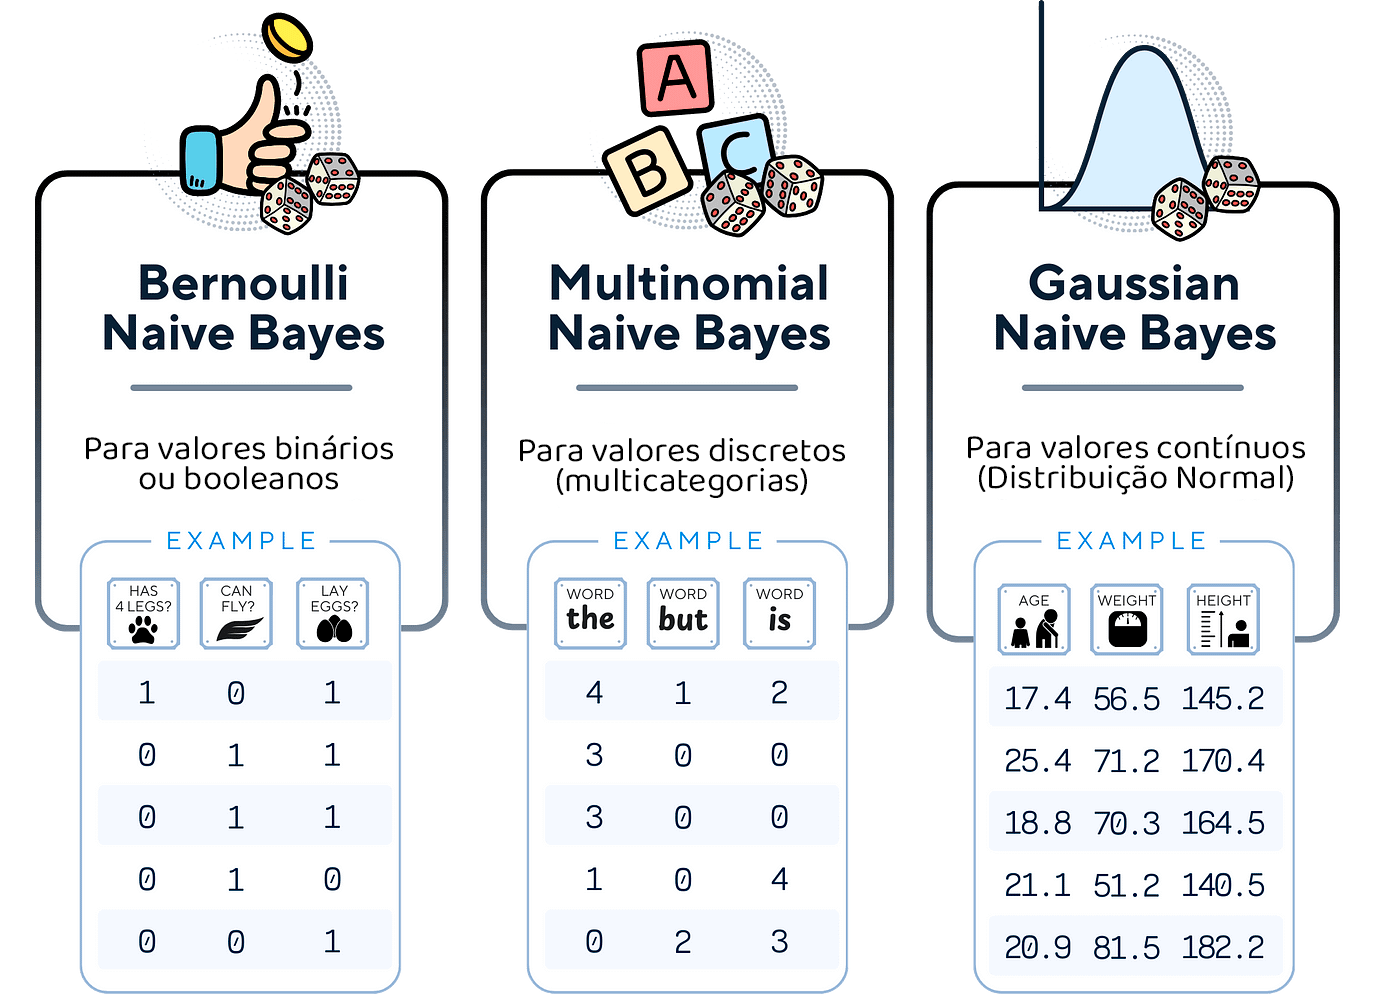
\includegraphics[width=0.5\linewidth]{img/naivebayes.png}
    \end{figure}
\end{frame}

\begin{frame}
    \frametitle{Árvore de Decisão (Decision Trees)}
    \begin{itemize}
        \item Vários pontos de decisão serão criados (nós).
        \item Em cada nó, o resultado da decisão será seguir por um caminho, ou por outro.
        \item  Uma pergunta será feita e teremos duas opções de resposta: sim ou não. A opção “sim” levará a uma próxima pergunta, e a opção “não” a outra.
    \end{itemize}
    \begin{figure}
        \centering
        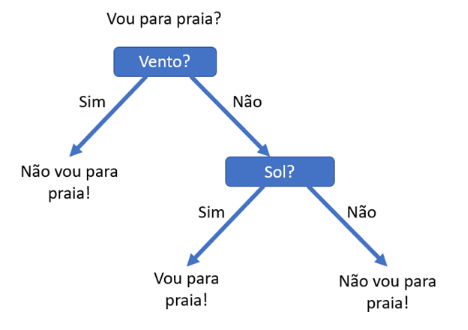
\includegraphics[width=0.5\linewidth]{img/ArvoreDecisao.png}
    \end{figure}
\end{frame}

\begin{frame}
    \frametitle{Floresta Aleatória (Random Florest)}
    \begin{itemize}
        \item Técnica de ensemble, ou seja, combina vários modelos para produzir um modelo final mais robusto.
        \item Constrói múltiplas Árvores de Decisão durante o treinamento e faz a média das previsões para melhorar a precisão e controlar o overfitting.
    \end{itemize}
    \begin{figure}
        \centering
        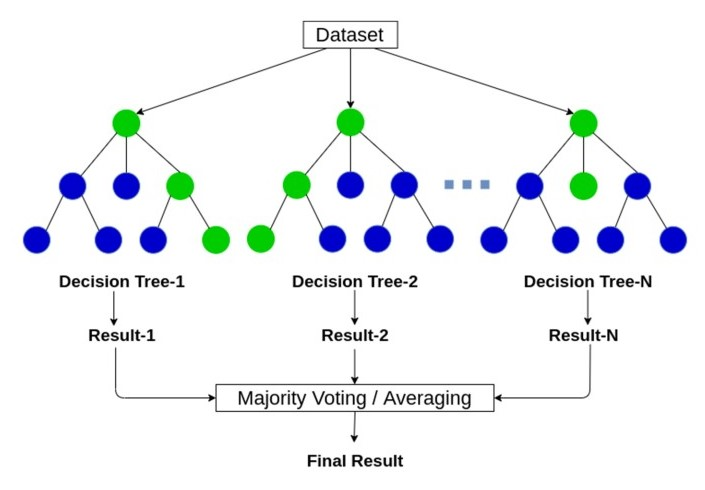
\includegraphics[width=0.5\linewidth]{img/randomflorest.jpeg}
    \end{figure}
\end{frame}

\section{Não Supervisionado} 

\begin{frame}
    \frametitle{Aprendizado Não Supervisionado}
    \begin{figure}
        \centering
        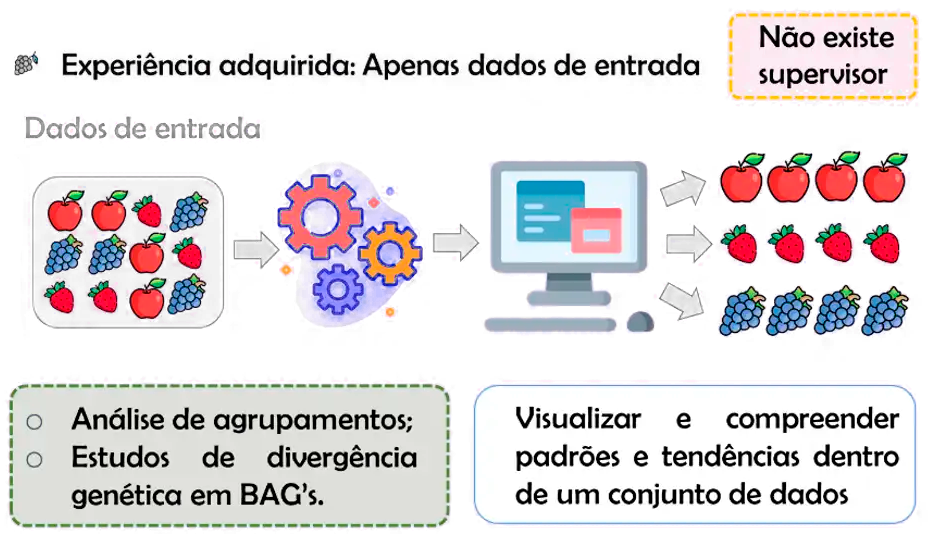
\includegraphics[width=1\linewidth]{img/nao-supervisionado.png}
    \end{figure}
\end{frame}

\begin{frame}
    \frametitle{Agrupamento}
    \begin{itemize}
        \item Identificar e agrupar dados semelhantes com base em características.
        \item O modelo organiza os dados em grupos (clusters) sem rótulos predefinidos.
    \end{itemize}

    \begin{figure}
        \centering
        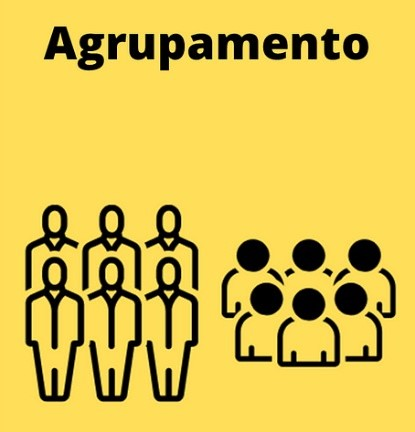
\includegraphics[width=0.3\linewidth]{img/agrupamento.jpg}
        \hspace{0.3cm}
        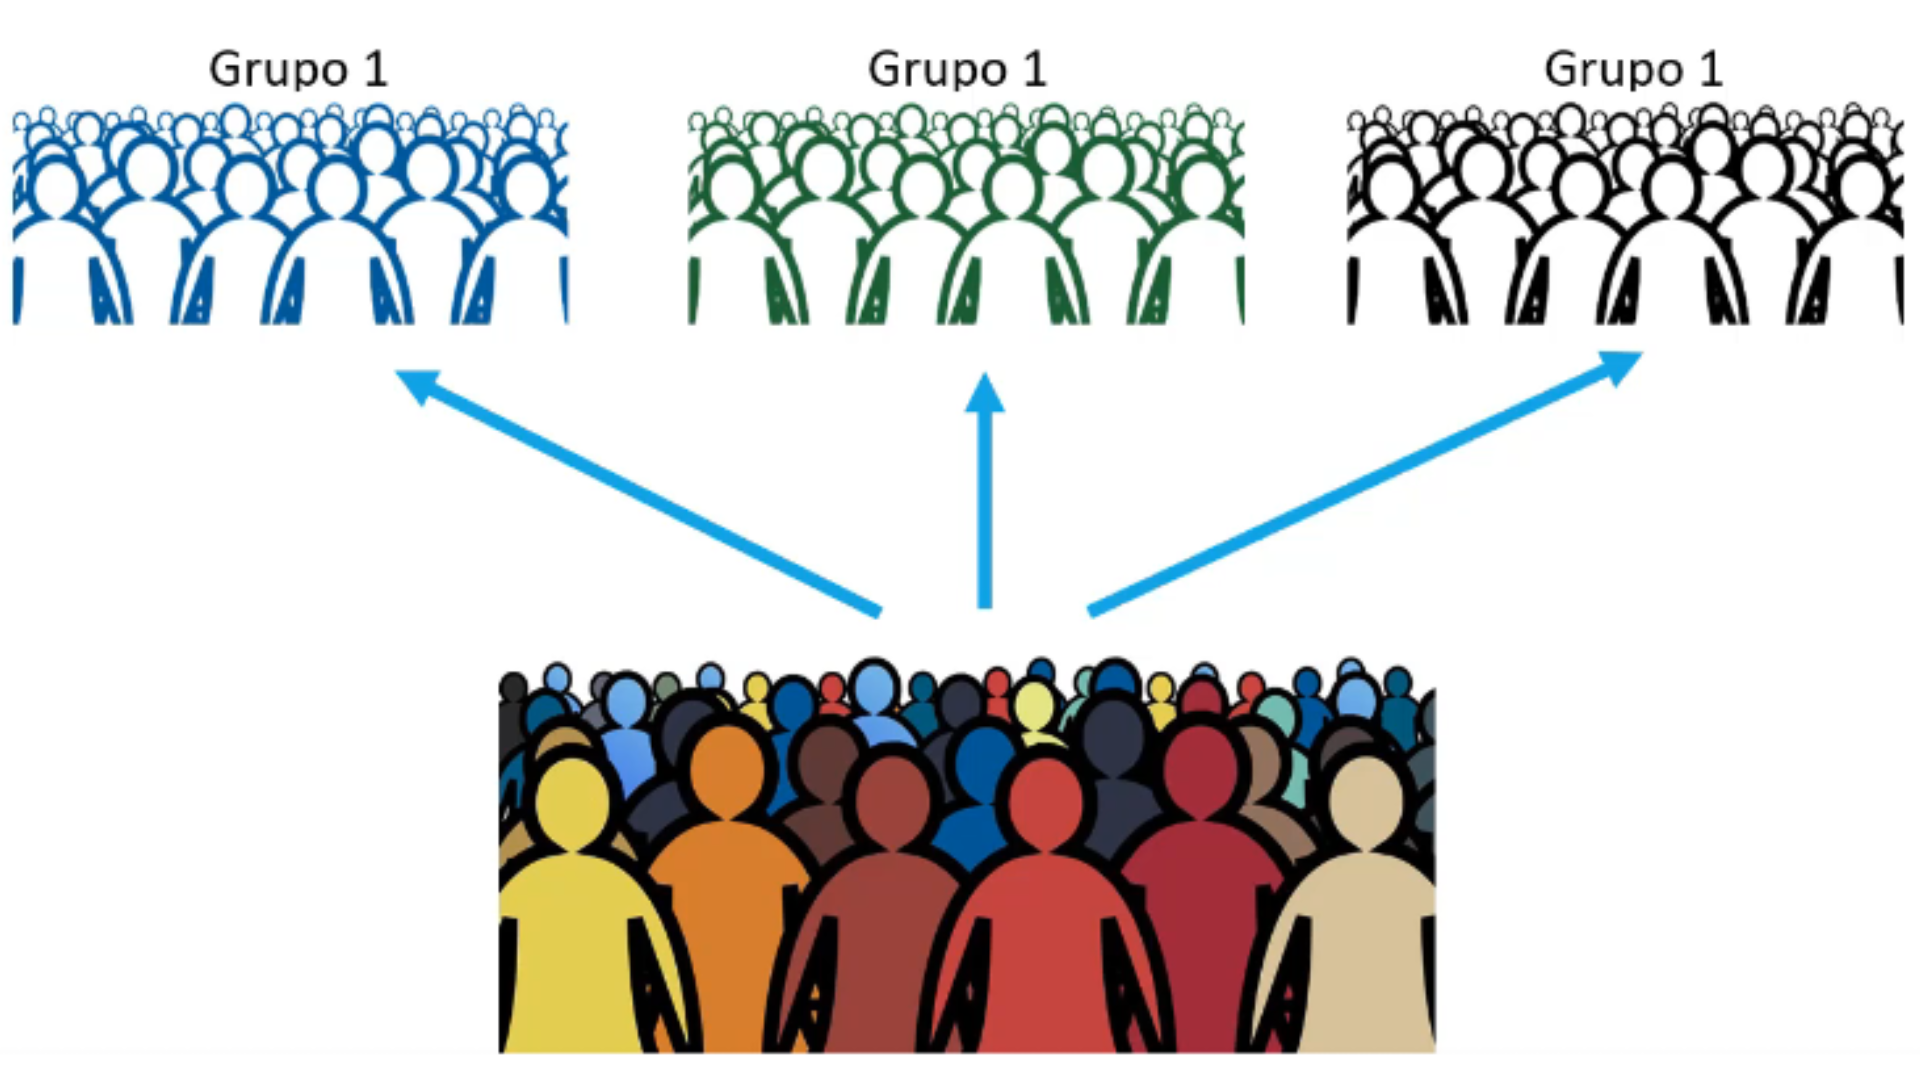
\includegraphics[width=0.6\linewidth]{img/agrupamento.png}
    \end{figure}
\end{frame}

\begin{frame}
    \frametitle{Agrupamento}
    \textbf{Exemplos:}
    \begin{itemize}
        \item \textbf{Segmentação de Clientes:} Agrupar clientes com comportamentos similares para personalização de campanhas (ex.: consumidores frequentes e esporádicos).
        
        \item \textbf{Agrupamento de Imagens:} Organizar imagens com base em semelhanças visuais (ex.: agrupar fotos de paisagens, animais ou objetos).

        \item \textbf{Agrupamento de Dados Geoespaciais:} Agrupar cidades, bairros e regiões com base em características socioeconômicas (renda, mobilidade, infraestrutura) ou ambientais (tipo de solo, cobertura florestal, disponibilidade de água)
    \end{itemize}
\end{frame}

\begin{frame}
    \frametitle{Algoritmos K-Means}
    \begin{itemize}
        \item "K" = Número de centroides (clusters) definidos previamente
        \item  “Means” = Média dos pontos em cada cluster. Determina a posição de seu centroide.
    \end{itemize}
    .
    \begin{figure}
        \centering
        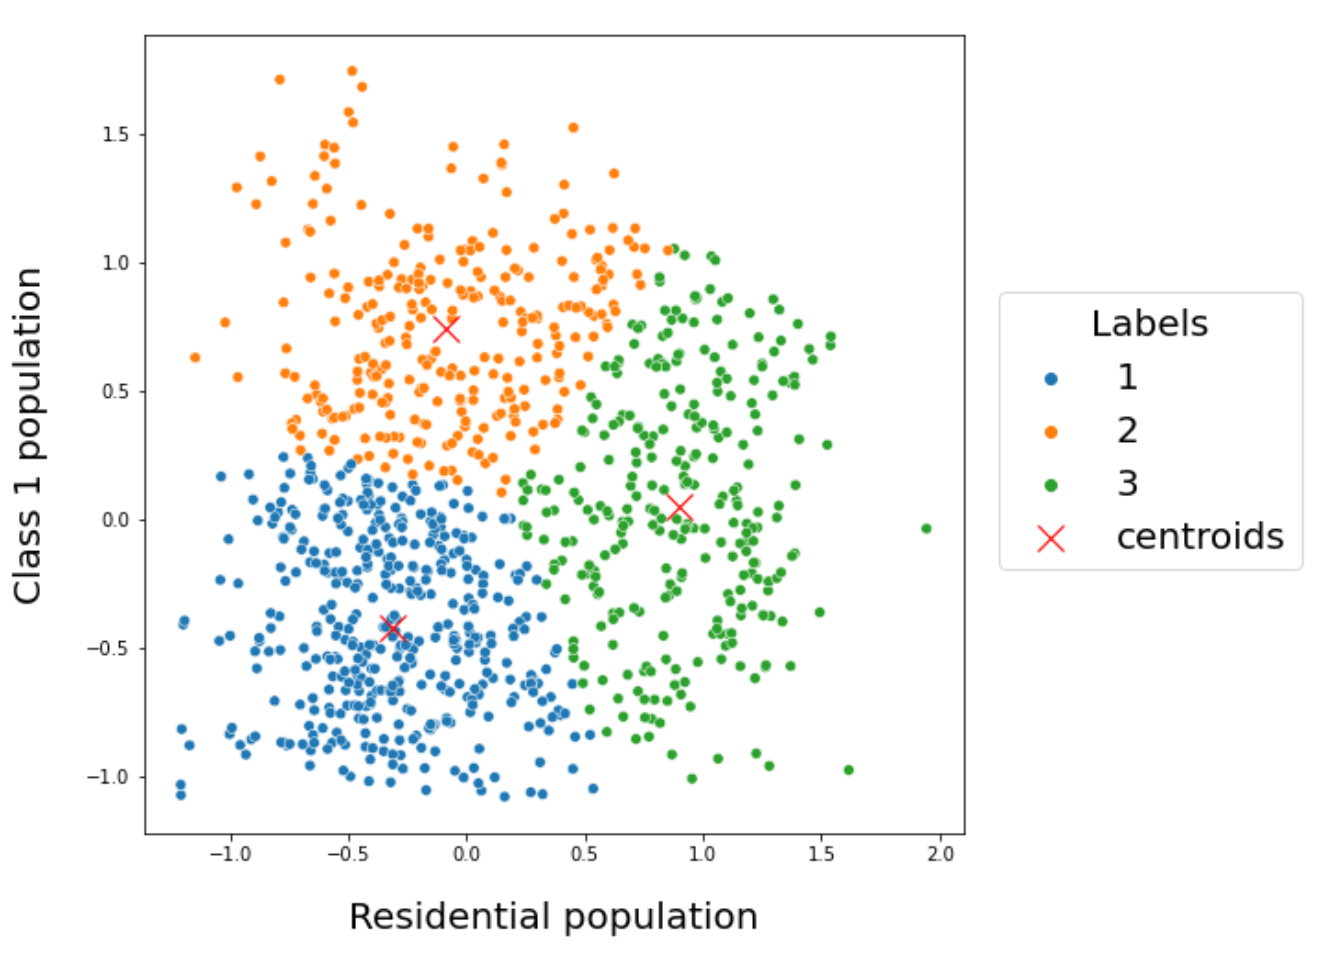
\includegraphics[width=0.5\linewidth]{img/imagekmeans.png}
    \end{figure}
\end{frame}

\begin{frame}
    \frametitle{Algoritmos K-Means}
    \begin{itemize}
        \item Os centroides são posicionado na média dos pontos pertencentes ao seu cluster.
        \item O algoritmo encontra o centroide mais próximo a um novo ponto.
        \item O ponto é então classificado como \textbf{pertencente ao cluster} daquele centroide.
    \end{itemize}
    \begin{figure}
        \centering
        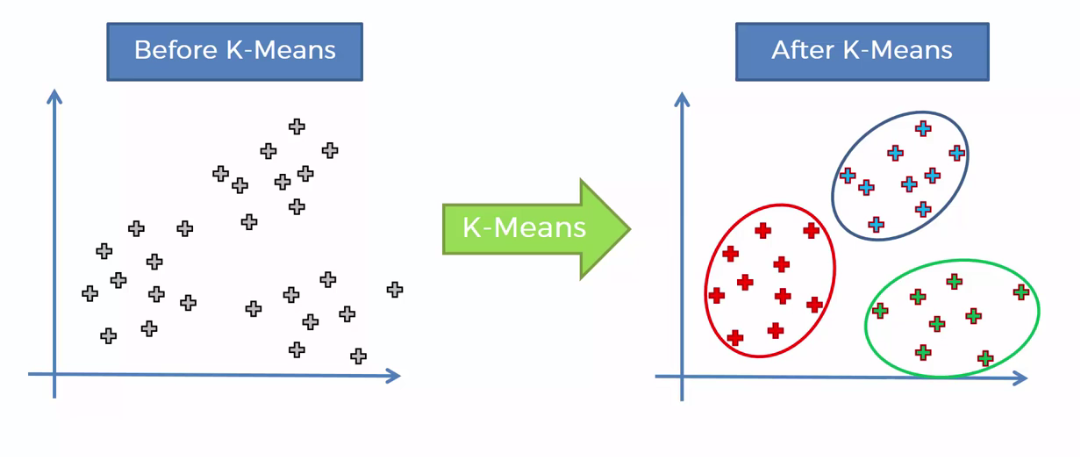
\includegraphics[width=0.5\linewidth]{img/kmeans.png}
    \end{figure}
\end{frame}

\begin{frame}
    \frametitle{Métricas de Avaliação do Agrupamento}
    \textbf{Inércia (Coesão):}
    \begin{itemize}
        \item Mede \textbf{o quão próximos os pontos estão} dentro de um mesmo cluster.
        \item Menores valores =  maior densidade.
        \item Menor distância entre os pontos dentro de um cluster = \textbf{maior a inércia} e mais \textbf{similares} são entre si.
    \end{itemize}

    \textbf{Separação:}
    \begin{itemize}
        \item Avalia a \textbf{distãncia} entre clusters.
        \item Valores maiores = os clusters estão bem separados.
        \item Um \textbf{bom} agrupamento deve ter \textbf{uma alta separação}, significando que os clusters não estão se sobrepondo e são bem distintos entre si.
    \end{itemize}
\end{frame}

\begin{frame}
    \frametitle{Coeficiente de Silhueta (Silhouette Score)}
    \begin{itemize}
        \item Combina a inércia e a separação para fornecer uma \textbf{visão balanceada} da clusterização;
        \item O valor dessa métrica varia de -1 a 1, \item Valor negativo indica que o ponto pode ter sido atribuído ao cluster errado.
    \end{itemize}
    
     \begin{center}
    \[
    Silhueta_{\,\textit{ponto i}} = \frac{\textit{Inercia}_{i} - \textit{Separação}_{i}}{max(\textit{Inércia}_{i}, \textit{Separação}_{i})}
    \]
    \end{center}

\end{frame}

\begin{frame}
    \frametitle{Método do Cotovelo}
    \begin{itemize}
        \item Determina o número ideal de clusters identificando o ponto onde a redução na inércia se torna marginal.
    \end{itemize}

    \begin{figure}
        \centering
        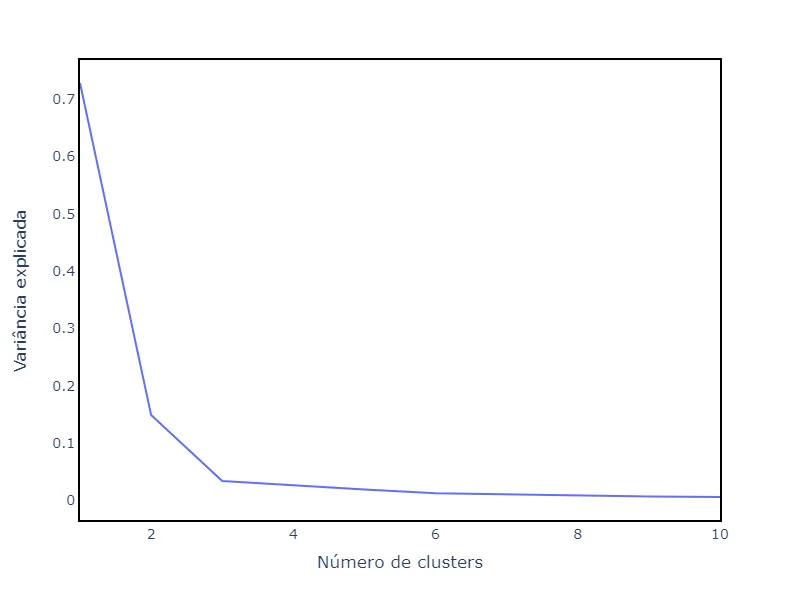
\includegraphics[width=0.6\linewidth]{img/imagecotovelo.png}
    \end{figure}
\end{frame}
\section{Validação de Modelos} 

\begin{frame}
    \frametitle{Overfitting (Sobreajuste)}
    \begin{itemize}
        \item Previsões precisas para dados de \textbf{treinamento}, mas não para \textbf{novos dados}.
    \end{itemize}
    \vspace{0.3cm}
    \textbf{Alguns motivos:}
    \begin{itemize}
        \item O tamanho dos dados de treinamento é muito pequeno.
        \item Dados de treinamento com grandes quantidades de informações irrelevantes.
        \item O modelo treina por muito tempo em um único conjunto de dados.
        \item  A \textbf{complexidade} do modelo é \textbf{alta}, então ele aprende o ruído nos dados de treinamento.
    \end{itemize}
\end{frame}

\begin{frame}
    \frametitle{Underfitting (Subajuste)}
    \begin{itemize}
        \item O modelo não pode determinar uma relação significativa entre os dados de entrada e saída.
        \item Fornecem resultados imprecisos tanto para os \textbf{dados de treinamento} quanto para o \textbf{conjunto de testes}.
    \end{itemize}
    \begin{figure}
        \centering
        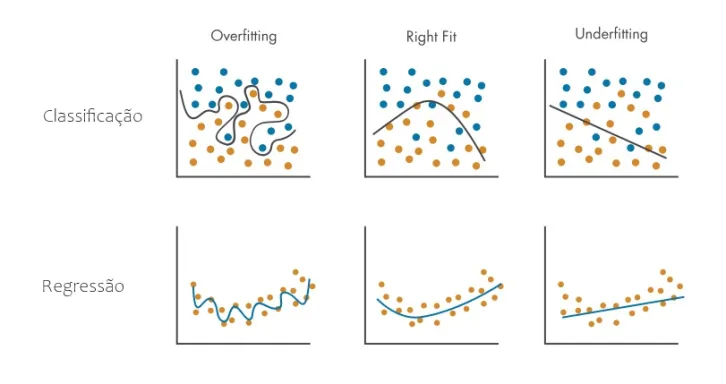
\includegraphics[width=0.8\linewidth]{img/imageoverunder.png}
    \end{figure}
\end{frame}

\begin{frame}
    \frametitle{Validação de Modelos}
    A fase de testar o nosso modelo!
    \begin{itemize}
        \item A validação de modelos avalia o desempenho de um modelo em dados não vistos durante o treinamento.
        \item Garante que o modelo generalize bem para dados do mundo real.
        \item Evita problemas como overfitting (superajuste) e underfitting (subajuste).
\end{itemize}
    
    \textbf{Técnicas comuns:}
    \begin{itemize}
            \item Divisão Treino/Validação/Teste (Hold-out)
            \item Validação Cruzada (Cross-Validation)
    \end{itemize}
\end{frame}

\begin{frame}
    \frametitle{Hold-Out}
    \begin{itemize}
        \item Divide o dataset, separando os dados para o Treinamento e para o Teste do modelo.
    \end{itemize}
    \begin{figure}
        \centering
        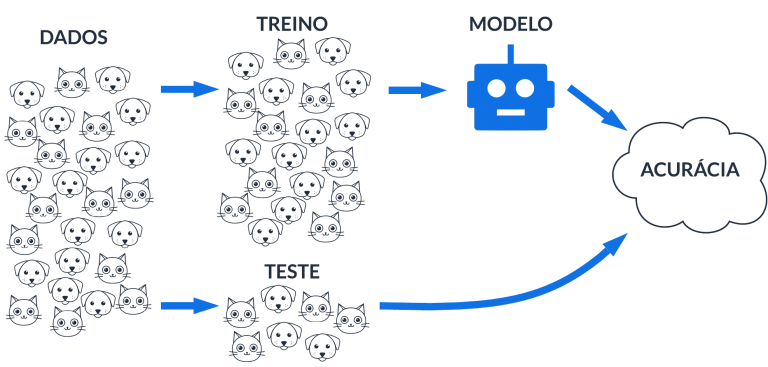
\includegraphics[width=0.8\linewidth]{img/imageholdout.png}
    \end{figure}
\end{frame}

\begin{frame}
    \frametitle{Hold-Out}
    \begin{itemize}
        \item Para modelos mais complexos os dados de treinamento são novamente divididos entre Treino e Validação, para ser possível fazer ajustes no modelo sem utilizar dos dados de Teste.
    \end{itemize}
    \begin{figure}
        \centering
        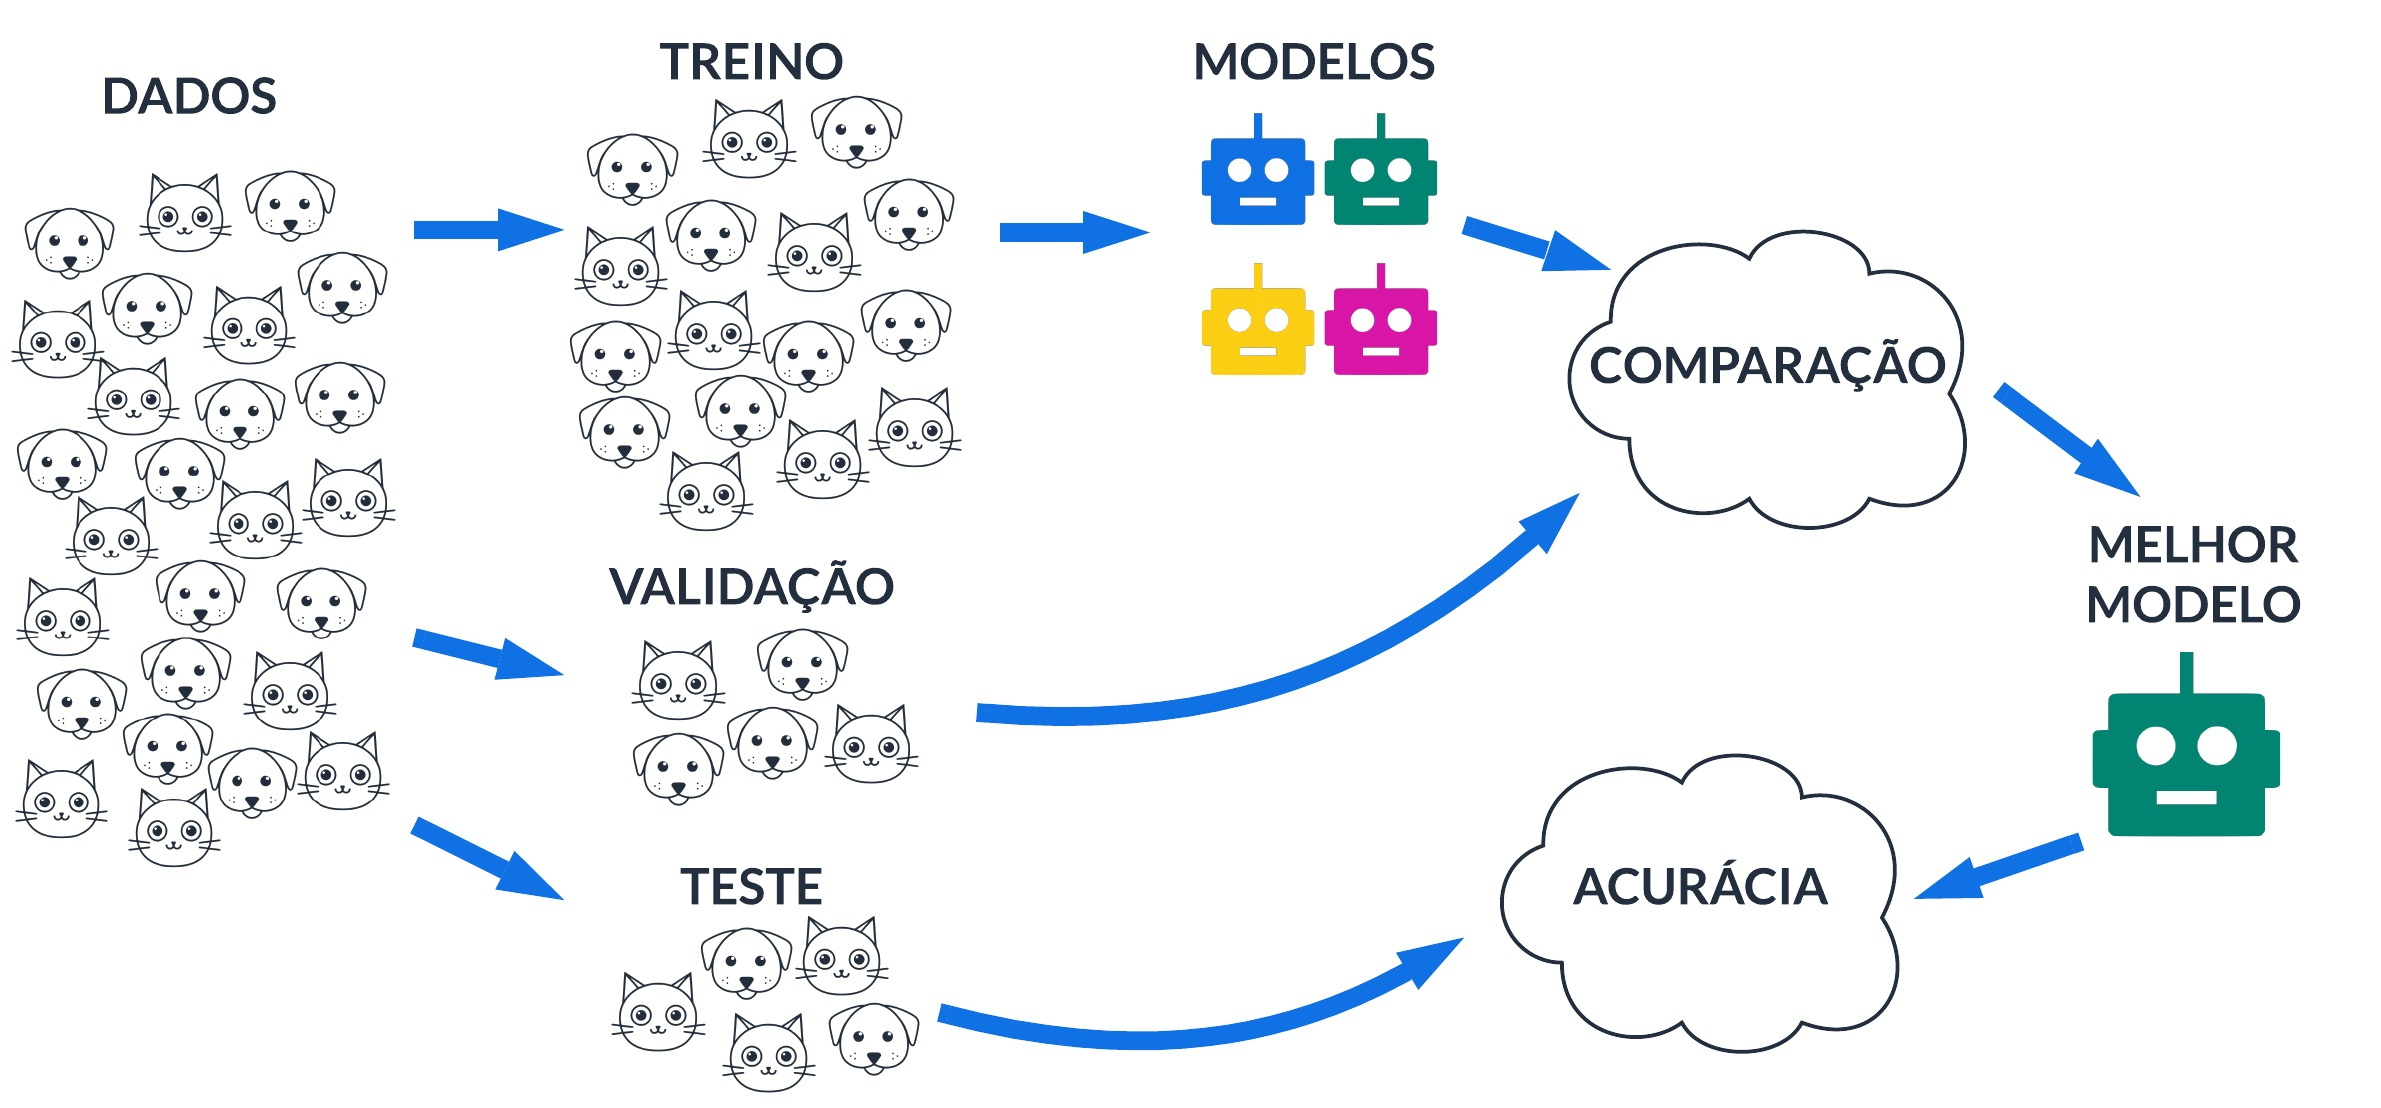
\includegraphics[width=0.8\linewidth]{img/image-ttv.png}
    \end{figure}
\end{frame}

\begin{frame}
    \frametitle{Validação Cruzada (K-fold)}
    
    \begin{itemize}
        \item Divide os dados em múltiplos subconjuntos (folds).
        \item Treina o modelo em \( k-1 \) folds e testa no fold restante.
        \item Processo repetido \( k \) vezes, garantindo que todos os dados sejam usados para treino e teste.
    \end{itemize}

    \begin{figure}
        \centering
        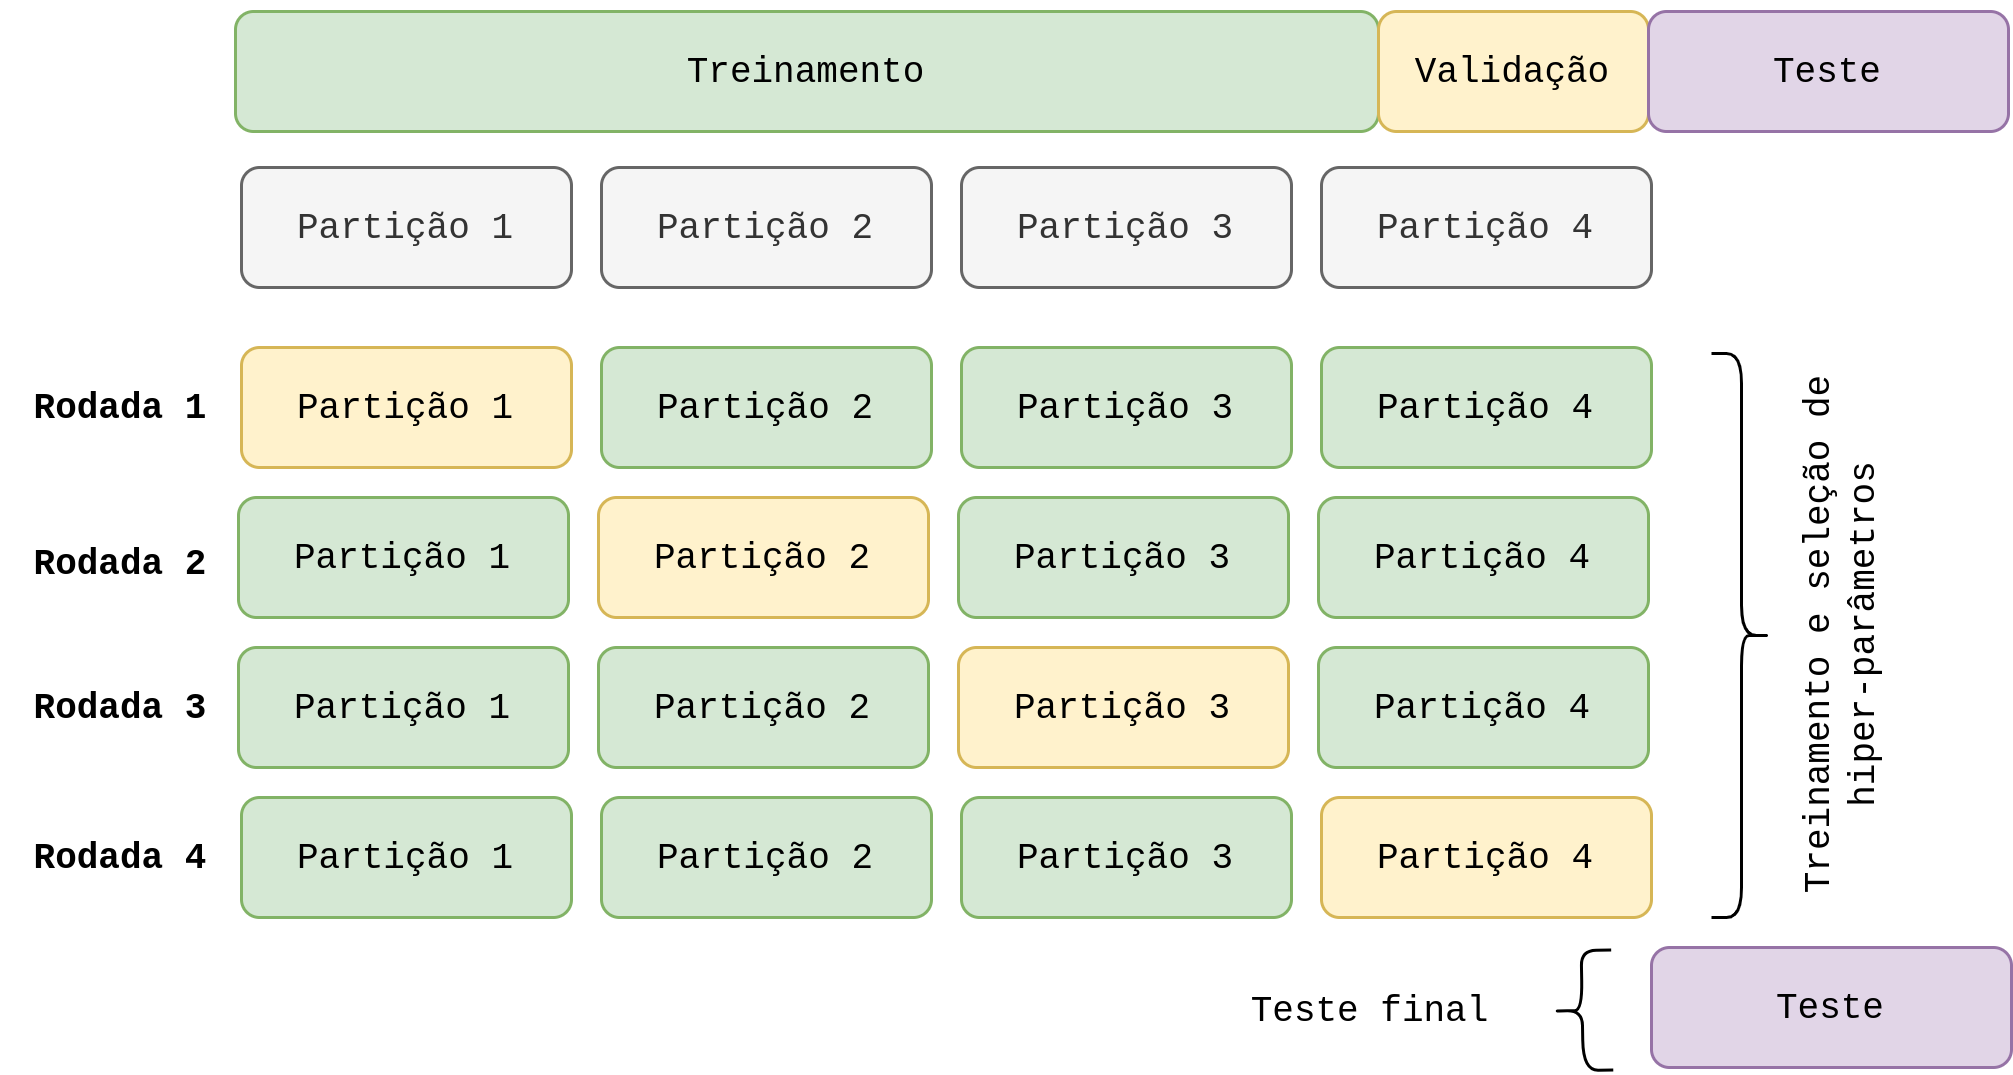
\includegraphics[width=0.7\linewidth]{img/cross_val.png}
    \end{figure}
\end{frame}
\section{Scikit-Learn}
\begin{frame}
	\frametitle{Oque é?}	
	\centering
	\begin{itemize}
		\item O scikit-learn é uma biblioteca feita para simplificar o treinamento e uso de modelos de machine learning em Python
	\end{itemize}
	
\includegraphics[width=0.3\linewidth]{Scikit_learn_logo.png}
	
\includegraphics[width=0.3\linewidth]{python_logo.png}
\end{frame}
\begin{frame}
	\frametitle{Principais características}	
	\begin{itemize}
		\item Ideal para modelos de ML clássicos
		\item Ferramentas simples de pré-processamento, treino e validação
		\item API simples de usar
		\item Integração nativa com outras bibliotecas do python
	\end{itemize}
	\centering
	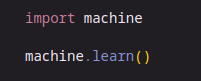
\includegraphics[width=0.25\linewidth]{eh_isso_que_eh_machine_learning?.png}
\end{frame}
\begin{frame}
	\frametitle{Oque vamos abordar}	
	\begin{itemize}
		\item Vamos ver como o tratamento e pré-processamento dos dados é uma camada importante no processo de aprendizado de máquina
		\item Vamos abordar os métodos para uso em código dos algoritmos de treino supervisionado e não supervisionado vistos
	\end{itemize}
\end{frame}
%----------------------------------------------------------------------------------------
%	SLIDE DE ENCERRAMENTO
%----------------------------------------------------------------------------------------

\begin{frame}
    \begin{center}
    \begin{figure}
        
\includegraphics[width=0.30\linewidth]{img/GETlogo_azul.png}
    \end{figure}
    \vspace{0.5cm}
    {\Huge Obrigado pela atenção!}
    \end{center}
\end{frame}

%----------------------------------------------------------------------------------------

\end{document}
